\documentclass[../mathNotesPreamble]{subfiles}
\begin{document}
%\relscale{1.4} %TODO
\section{15.8: Lagrange Multipliers}
  Constrained optimization functions have an \textbf{objective function} $f$ with the restriction that the independent variables $x$ and $y$ lie on a \textbf{constraint} curve $C$ in the $xy$-plane given by $g(x,y)=0$.
  \vspace*{\stretch{1}}

  \begin{center}
    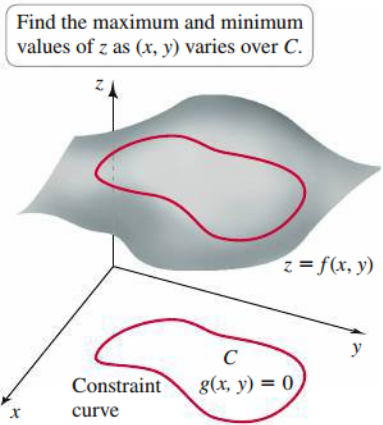
\includegraphics[width=0.3\linewidth]{../images/briggs_15_08/fig15_79}
    \hspace*{20mm}
    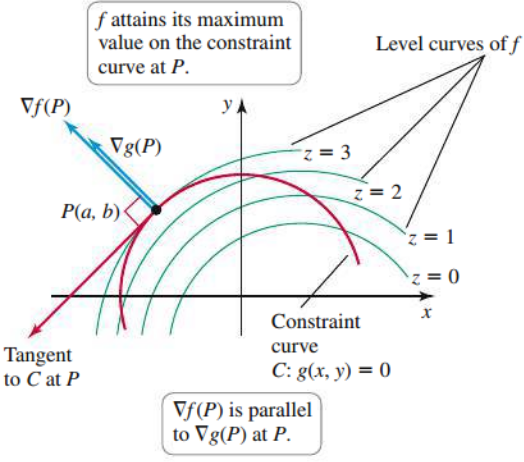
\includegraphics[width=0.375\linewidth]{../images/briggs_15_08/fig15_80}
  \end{center}
  \vspace*{\stretch{1}}

  \begin{defn*}[Parallel Gradients]
    Let $f$ be a differentiable function in a region of $\bbr^2$ that contains the smooth curve $C$ given by $g(x,y)=0$. Assume $f$ has a local extreme value on $C$ at a point $P(a,b)$. Then $\grad f(a,b)$ is orthogonal to the line tangent to $C$ at $P$. Assuming $\grad g(a,b)\neq \bfO$, it follows that there is a real number $\lambda$ (called a \textbf{Lagrange multiplier}) such that $\grad f(a,b)=\lambda \grad g(a,b)$.
  \end{defn*}

  We consider the three following cases:
  \begin{tasks}[label=\textbullet](1)
    \task 
      Bounded constraint curves that close on themselves (e.g. circles, ellipses, etc),
    \task 
      Bounded constraint curves that do not close on themselves, but include endpoints,
    \task 
      Unbounded constraint curves
  \end{tasks}
  \pagebreak

  \begin{ex*}
    Find the absolute maximum and minimum values of the objective function $f(x,y)=x^2+y^2+2$, where $x$ and $y$ lie on the ellipse $C$ given by $g(x,y)=x^2+xy+y^2-4=0$.
  \end{ex*}
  \vspace*{\stretch{1}}
  \begin{flushright}
    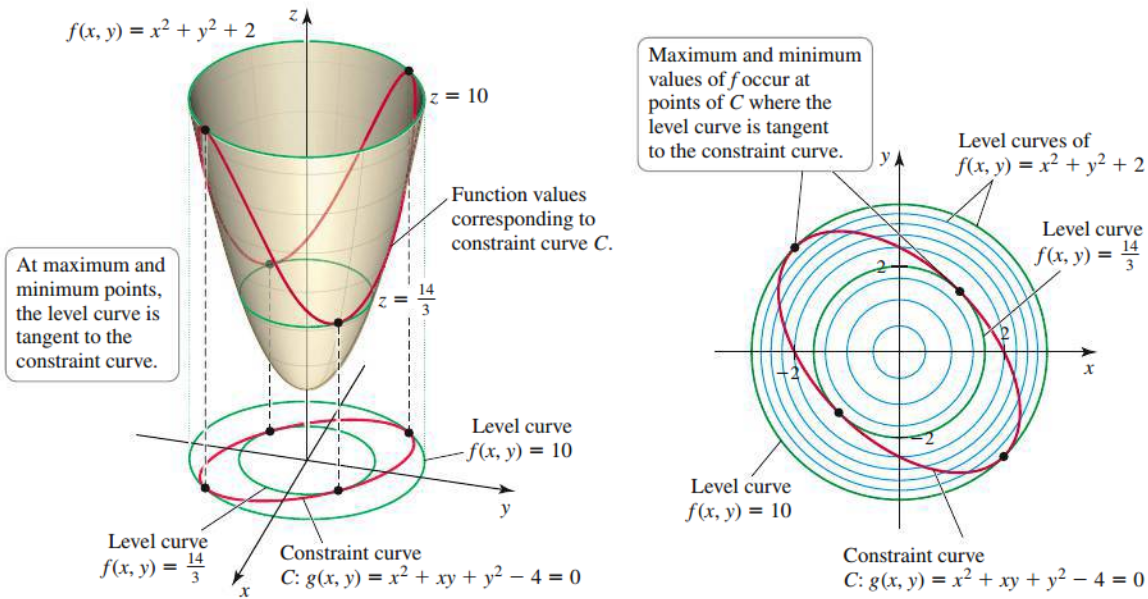
\includegraphics[width=0.65\linewidth]{../images/briggs_15_08/fig15_81}
  \end{flushright}
  \pagebreak

  \begin{thmBox*}[Procedure- Lagrange Multipliers: Absolute Extrema on Closed and \newline Bounded Constraint Curves]
    Let the objective function $f$ and the constraint function $g$ be differentiable on a region $\bbr^2$ with $\grad g(x,y)\neq\bfO$ on the curve $g(x,y)=0$. To locate the absolute maximum and minimum values of $f$ subject to the constraint $g(x,y)=0$, carry out the following steps.
    \begin{enumerate}
      \item 
        Find the values of $x$, $y$, and $\lambda$ (if they exist) that satisfy the equations
          \[\grad f(x,y)=\lambda \grad g(x,y) \textnormal{ and } g(x,y)=0.\]
      \item 
        Evaluate $f$ at the values $(x,y)$ in Step 1 and at the endpoints of the constraint curve (if they exist). Select the largest and smallest corresponding function values. These values are the absolute maximum and minimum values of $f$ subject to the constraint.
    \end{enumerate}
  \end{thmBox*}

  \noindent
  Using Lagrange multipliers extends to higher dimensions with three or more independent variables:
  \begin{center}
    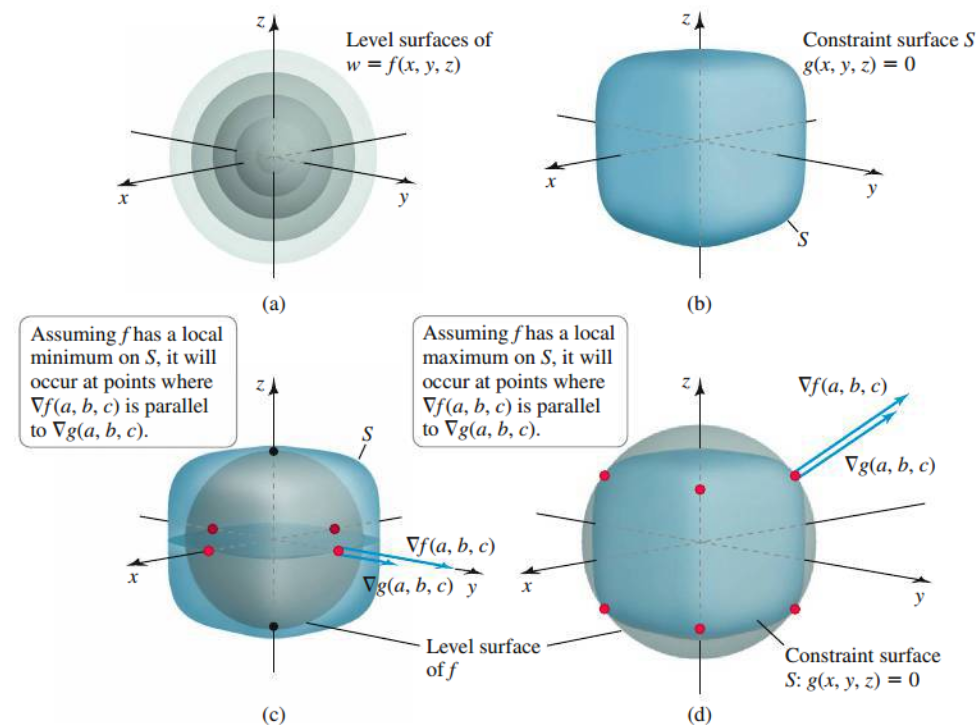
\includegraphics[width=0.605\linewidth]{../images/briggs_15_08/fig15_82}
  \end{center}
  \pagebreak

  \begin{ex*}
    Find the least distance between the point $P(3,4,0)$ and the surface of the cone $z^2=x^2+y^2$.
  \end{ex*}
  \vspace*{\stretch{1}}
  \pagebreak

  \begin{ex*}
    Find the absolute maximum value of the utility function $U=f(\ell,g)=\ell^{1/3} g^{2/3}$, subject to the constraint $G(\ell, g)=3\ell+2g-12=0$, where $\ell\geq 0$ and $g\geq 0$.
  \end{ex*}
  \vspace*{\stretch{1}}
  \pagebreak

  \begin{ex*}
    Find the maximum value of $x_1+x_2+x_3+x_4$ subject to the condition that $x_1^2+x_2^2+x_3^2+x_4^2=16$.
  \end{ex*}
  \vspace*{\stretch{1}}
  \pagebreak

  \begin{thmBox*}[Procedure- Lagrange Multipliers: Absolute Extrema on Closed and \newline Bounded Constraint Surfaces]
    Let $f$ and $g$ be differentiable on a region of $\bbr^3$ with $\grad g(x,y,z)\neq \bfO$ on the surface $g(x,y,z)=0$. To locate the absolute maximum and minimum values of $f$ subject to the constraint $g(x,y,z)=0$, carry out the following steps.
    \begin{enumerate}
      \item 
        Find the values of $x$, $y$, $z$, and $\lambda$ that satisfy the equations
          \[\grad f(x,y,z)=\lambda\grad g(x,y,z)\textnormal{ and } g(x,y,z)=0.\]
      \item 
        Among the points $(x,y,z)$ found in Step 1, select the largest and smallest corresponding function values. These values are the absolute maximum and minimum values of $f$ subject to the constraint.
    \end{enumerate}
  \end{thmBox*}

  \pagebreak
  
\end{document}
